\documentclass{standalone}
\usepackage{tikz}
\usetikzlibrary{patterns, positioning}

\begin{document}
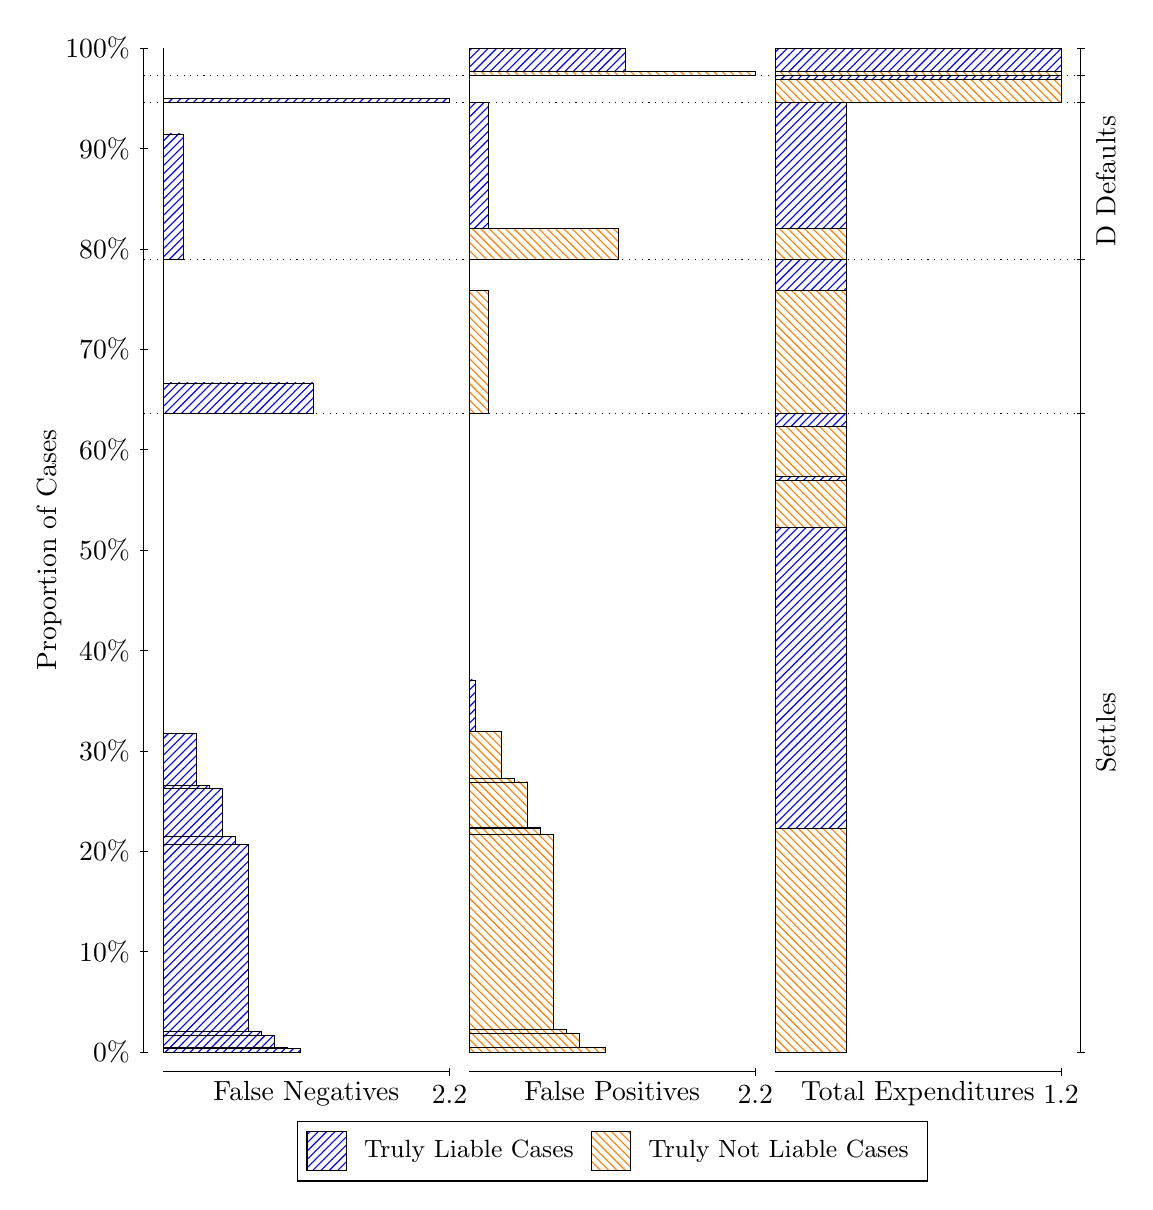
\begin{tikzpicture}
\draw[black, very thin] (1.5,1.75) -- (1.5,14.5);
\node[rotate=90, anchor=center] at (0.3, 8.125) {Proportion of Cases};
\draw[black, very thin] (1.45,1.75) -- (1.55,1.75);
\node[anchor=east] at (1.45, 1.75) {0\%};
\draw[black, very thin] (1.45,3.025) -- (1.55,3.025);
\node[anchor=east] at (1.45, 3.025) {10\%};
\draw[black, very thin] (1.45,4.3) -- (1.55,4.3);
\node[anchor=east] at (1.45, 4.3) {20\%};
\draw[black, very thin] (1.45,5.575) -- (1.55,5.575);
\node[anchor=east] at (1.45, 5.575) {30\%};
\draw[black, very thin] (1.45,6.85) -- (1.55,6.85);
\node[anchor=east] at (1.45, 6.85) {40\%};
\draw[black, very thin] (1.45,8.125) -- (1.55,8.125);
\node[anchor=east] at (1.45, 8.125) {50\%};
\draw[black, very thin] (1.45,9.4) -- (1.55,9.4);
\node[anchor=east] at (1.45, 9.4) {60\%};
\draw[black, very thin] (1.45,10.675) -- (1.55,10.675);
\node[anchor=east] at (1.45, 10.675) {70\%};
\draw[black, very thin] (1.45,11.95) -- (1.55,11.95);
\node[anchor=east] at (1.45, 11.95) {80\%};
\draw[black, very thin] (1.45,13.225) -- (1.55,13.225);
\node[anchor=east] at (1.45, 13.225) {90\%};
\draw[black, very thin] (1.45,14.5) -- (1.55,14.5);
\node[anchor=east] at (1.45, 14.5) {100\%};

\draw[black, very thin] (13.4,1.75) -- (13.4,14.5);
\draw[black, very thin] (13.35,1.75) -- (13.45,1.75);
\node[anchor=west] at (13.35, 1.75) {};
\draw[black, very thin] (13.35,9.8595) -- (13.45,9.8595);
\node[anchor=west] at (13.35, 9.8595) {};
\draw[black, very thin] (13.35,11.812) -- (13.45,11.812);
\node[anchor=west] at (13.35, 11.812) {};
\draw[black, very thin] (13.35,13.812) -- (13.45,13.812);
\node[anchor=west] at (13.35, 13.812) {};
\draw[black, very thin] (13.35,14.154) -- (13.45,14.154);
\node[anchor=west] at (13.35, 14.154) {};
\draw[black, very thin] (13.35,14.5) -- (13.45,14.5);
\node[anchor=west] at (13.35, 14.5) {};

\draw[black, very thin, pattern color=blue, pattern=north east lines] (1.75,1.75) rectangle (3.4841,1.8004);
\draw[black, very thin, pattern color=blue, pattern=north east lines] (1.75,1.8004) rectangle (3.3189,1.8067);
\draw[black, very thin, pattern color=blue, pattern=north east lines] (1.75,1.8067) rectangle (3.1538,1.9601);
\draw[black, very thin, pattern color=blue, pattern=north east lines] (1.75,1.9601) rectangle (2.9886,2.0164);
\draw[black, very thin, pattern color=blue, pattern=north east lines] (1.75,2.0164) rectangle (2.8235,4.39);
\draw[black, very thin, pattern color=blue, pattern=north east lines] (1.75,4.39) rectangle (2.6583,4.4928);
\draw[black, very thin, pattern color=blue, pattern=north east lines] (1.75,4.4928) rectangle (2.4932,5.0979);
\draw[black, very thin, pattern color=blue, pattern=north east lines] (1.75,5.0979) rectangle (2.328,5.1353);
\draw[black, very thin, pattern color=blue, pattern=north east lines] (1.75,5.1353) rectangle (2.1629,5.7922);
\draw[black, very thin, pattern color=orange, pattern=north west lines] (1.75,5.7922) rectangle (1.75,9.8595);
\draw[black, very thin, pattern color=blue, pattern=north east lines] (1.75,9.8595) rectangle (3.6492,10.247);
\draw[black, very thin, pattern color=orange, pattern=north west lines] (1.75,10.247) rectangle (1.75,11.812);
\draw[black, very thin, pattern color=blue, pattern=north east lines] (1.75,11.812) rectangle (1.9977,13.41);
\draw[black, very thin, pattern color=orange, pattern=north west lines] (1.75,13.41) rectangle (1.75,13.812);
\draw[black, very thin, pattern color=blue, pattern=north east lines] (1.75,13.812) rectangle (5.3833,13.864);
\draw[black, very thin, pattern color=orange, pattern=north west lines] (1.75,13.864) rectangle (1.75,14.154);
\draw[black, very thin, pattern color=orange, pattern=north west lines] (1.75,14.154) rectangle (1.75,14.206);
\draw[black, very thin, pattern color=blue, pattern=north east lines] (1.75,14.206) rectangle (1.75,14.5);
\draw[black, very thin, pattern color=orange, pattern=north west lines] (5.6333,1.75) rectangle (7.3674,1.8069);
\draw[black, very thin, pattern color=orange, pattern=north west lines] (5.6333,1.8069) rectangle (7.2023,1.813);
\draw[black, very thin, pattern color=orange, pattern=north west lines] (5.6333,1.813) rectangle (7.0371,1.9815);
\draw[black, very thin, pattern color=orange, pattern=north west lines] (5.6333,1.9815) rectangle (6.872,2.0415);
\draw[black, very thin, pattern color=orange, pattern=north west lines] (5.6333,2.0415) rectangle (6.7068,4.5093);
\draw[black, very thin, pattern color=orange, pattern=north west lines] (5.6333,4.5093) rectangle (6.5417,4.5866);
\draw[black, very thin, pattern color=orange, pattern=north west lines] (5.6333,4.5866) rectangle (6.5417,4.6003);
\draw[black, very thin, pattern color=orange, pattern=north west lines] (5.6333,4.6003) rectangle (6.3765,5.1807);
\draw[black, very thin, pattern color=orange, pattern=north west lines] (5.6333,5.1807) rectangle (6.2114,5.2198);
\draw[black, very thin, pattern color=orange, pattern=north west lines] (5.6333,5.2198) rectangle (6.0462,5.8173);
\draw[black, very thin, pattern color=blue, pattern=north east lines] (5.6333,5.8173) rectangle (5.7159,6.4742);
\draw[black, very thin, pattern color=blue, pattern=north east lines] (5.6333,6.4742) rectangle (5.6333,9.8595);
\draw[black, very thin, pattern color=orange, pattern=north west lines] (5.6333,9.8595) rectangle (5.8811,11.424);
\draw[black, very thin, pattern color=blue, pattern=north east lines] (5.6333,11.424) rectangle (5.6333,11.812);
\draw[black, very thin, pattern color=orange, pattern=north west lines] (5.6333,11.812) rectangle (7.5326,12.213);
\draw[black, very thin, pattern color=blue, pattern=north east lines] (5.6333,12.213) rectangle (5.8811,13.812);
\draw[black, very thin, pattern color=orange, pattern=north west lines] (5.6333,13.812) rectangle (5.6333,14.103);
\draw[black, very thin, pattern color=blue, pattern=north east lines] (5.6333,14.103) rectangle (5.6333,14.154);
\draw[black, very thin, pattern color=orange, pattern=north west lines] (5.6333,14.154) rectangle (9.2667,14.206);
\draw[black, very thin, pattern color=blue, pattern=north east lines] (5.6333,14.206) rectangle (7.6152,14.5);
\draw[black, very thin, pattern color=orange, pattern=north west lines] (9.5167,1.75) rectangle (10.425,4.5866);
\draw[black, very thin, pattern color=blue, pattern=north east lines] (9.5167,4.5866) rectangle (10.425,8.4144);
\draw[black, very thin, pattern color=orange, pattern=north west lines] (9.5167,8.4144) rectangle (10.425,9.0119);
\draw[black, very thin, pattern color=blue, pattern=north east lines] (9.5167,9.0119) rectangle (10.425,9.0623);
\draw[black, very thin, pattern color=orange, pattern=north west lines] (9.5167,9.0623) rectangle (10.425,9.6955);
\draw[black, very thin, pattern color=blue, pattern=north east lines] (9.5167,9.6955) rectangle (10.425,9.8595);
\draw[black, very thin, pattern color=orange, pattern=north west lines] (9.5167,9.8595) rectangle (10.425,11.424);
\draw[black, very thin, pattern color=blue, pattern=north east lines] (9.5167,11.424) rectangle (10.425,11.812);
\draw[black, very thin, pattern color=orange, pattern=north west lines] (9.5167,11.812) rectangle (10.425,12.213);
\draw[black, very thin, pattern color=blue, pattern=north east lines] (9.5167,12.213) rectangle (10.425,13.812);
\draw[black, very thin, pattern color=orange, pattern=north west lines] (9.5167,13.812) rectangle (13.15,14.103);
\draw[black, very thin, pattern color=blue, pattern=north east lines] (9.5167,14.103) rectangle (13.15,14.154);
\draw[black, very thin, pattern color=orange, pattern=north west lines] (9.5167,14.154) rectangle (13.15,14.206);
\draw[black, very thin, pattern color=blue, pattern=north east lines] (9.5167,14.206) rectangle (13.15,14.5);
\draw[black, dotted] (1.5,9.8595) -- (13.4,9.8595);
\draw[black, dotted] (1.5,11.812) -- (13.4,11.812);
\draw[black, dotted] (1.5,13.812) -- (13.4,13.812);
\draw[black, dotted] (1.5,14.154) -- (13.4,14.154);
\draw[black, very thin] (1.75,1.5) -- (5.3833,1.5);
\node[anchor=north] at (3.5667, 1.5) {False Negatives};
\draw[black, very thin] (5.3833,1.45) -- (5.3833,1.55);
\node[anchor=north] at (5.3833, 1.45) {2.2};

\draw[black, very thin] (5.6333,1.5) -- (9.2667,1.5);
\node[anchor=north] at (7.45, 1.5) {False Positives};
\draw[black, very thin] (9.2667,1.45) -- (9.2667,1.55);
\node[anchor=north] at (9.2667, 1.45) {2.2};

\draw[black, very thin] (9.5167,1.5) -- (13.15,1.5);
\node[anchor=north] at (11.333, 1.5) {Total Expenditures};
\draw[black, very thin] (13.15,1.45) -- (13.15,1.55);
\node[anchor=north] at (13.15, 1.45) {1.2};

\node[black, centered, rotate=90] at (13.72, 5.8048) {Settles};

\node[black, centered, rotate=90] at (13.72, 12.812) {D Defaults};



\draw (7.449999999999999,1.5) node[draw=none] (baseCoordinate) {};
\begin{scope}[align=center]
        \matrix[scale=0.5, draw=black, below=0.5cm of baseCoordinate, nodes={draw}, column sep=0.1cm]{
            \node[rectangle, draw, minimum width=0.5cm, minimum height=0.5cm, pattern=north east lines, pattern color=blue] {}; &
            \node[draw=none, font=\small] (B) {Truly Liable Cases}; &
            \node[rectangle, draw, minimum width=0.5cm, minimum height=0.5cm, pattern=north west lines, pattern color=orange] {}; &
            \node[draw=none, font=\small] (B) {Truly Not Liable Cases}; \\
            };
\end{scope}

\end{tikzpicture}
\end{document}